\thispagestyle{plain}
\section{Results}
\indent

To verify the model implementation of both aforementioned models in MARS solver \cite{mars}, the numerically obtained data are compared to experimental measurements \cite{heinrich2012generation,Deuch_phd_thesis} and corresponding conclusions are drawn.


\subsection{Testing of Drucker-Prager model}
\indent
 
To verify the proper implementation and to check the ability of Drucker-Prager model to capture the behavior of thermoset polymers, the simple compression test of hybrid vinyl-ester mortar presented in \cite{Deuch_phd_thesis} is utilized. The test setup and specimen dimensions are shown in Fig. \ref{obr:test_param}. The material properties of this material presented also in \cite{Deuch_phd_thesis} at $\ang{25}\mathrm{C} $ are: $E = 6792~\mathrm{MPa}$; $\nu = 0.3$. Moreover, the parameters used for simulations using the Mohr-Coulomb yield criterion with an associated flow-rule in \cite{Deuch_phd_thesis} are: $\phi = \ang{28}$ and $c = 26.1~\mathrm{MPa}$. As can be seen in Fig. \ref{obr:Compresion_test}, linear 3D 8-node fine elements with 8 integration points are employed to discretize the specimen. To mimic the real setup, two rigid bodies (plates) are used to apply the load. The bottom plate is fixed in all directions and the rotation is not allowed, the top plate is fixed in horizontal directions and can rotate about horizontal axes. The load is applied by means of the prescribed displacement of the top plate in the vertical direction. The sliding with friction constraint is used for the contact between the specimen and plates, see \cite{mars} for more details. The general deformation of the specimen in the plastic regime is also presented in Fig. \ref{obr:Compresion_test}. 

\begin{figure}[h!]
	\centering
	\includegraphics[width=0.8\textwidth]{obrazky/test_parameters.png}
	\caption[Compression test parameters]{Compression test parameters \cite{Deuch_phd_thesis}: a) setup; b) specimen dimensions.}\label{obr:test_param}
\end{figure}

\begin{figure}[h!]
	\centering
	\includegraphics[width=0.8\textwidth]{obrazky/compression_displacement_magnitude.jpg}
	\caption[Compression test sample]{Compression test sample: on the surface you can see computed magnitude of displacement of the Drucker-Prager model without hardening of parameters.}\label{obr:Compresion_test}
\end{figure}


\begin{figure}[h!]
	\centering
	\includegraphics[width=1\textwidth]{obrazky/compression_test.eps}
	\caption[Compresion tests]{Compression tests compared to the real specimen result \cite{Deuch_phd_thesis}}\label{obr:Compresion_2d}
\end{figure}

The numerical results, obtained for different material parameters, are compared to the experimental data \cite{Deuch_phd_thesis} in Fig. \ref{obr:Compresion_2d}. The red line stands for the Drucker-Prager model, where $M_{JP}$ is computed according to Eq. (\ref{eq:f_Mjp_30}), the orange line represents the use of Eq. (\ref{eq:f_Mjp_-30}) and the purple line corresponds to $M_{JP}$ calculated according to Eq. (\ref{eq:f_Mjp_i}). All these simulations assume the parameters presented above, the associated flow-rule is also employed, i.e. $\psi=\phi$. The remaining simulations assume the evolution of cohesion with respect to $E_d^{pl}$ (hardening). The response for the evolution defined by $c=20\mathrm{MPa}$ for $E_d^{pl}=0$ and $c=40\mathrm{MPa}$ for $E_d^{pl}=0.05$ is represented by the green line in Fig. \ref{obr:Compresion_2d}. The updated evolution characterized by $c=15\mathrm{MPa}$ for $E_d^{pl}=0$ and $c=60\mathrm{MPa}$ for $E_d^{pl}=0.15$ is utilized to match the experimental data (light blue line). As can be seen, if the hardening is assumed, the numerical simulation adequately matches the experimental data. However, it has to be mentioned that the final conclusions cannot be drawn yet since only one loading scenario is utilized. To properly characterize the model suitability for studied thermoset polymers, additional experimental data are needed.  As mentioned in \cite{Deuch_phd_thesis}, the extension of Drucker-Prager model by Rankine failure criterion or compressive cap. 

Figs. \ref{obr:Compresion_parameters} – \ref{obr:Compresion_total_strain} show the distribution of model parameters, internal model variables and strains for the relative elongation $\Delta L/L = …$ of the material model with the hardening ($c=15$\,MPa for $E_d^{pl}=0$ and $c=60$\,MPa for $E_d^{pl}=0.15$ ). Fig. \ref{obr:Compresion_parameters} clearly demonstrate the prescribe constant value of friction angle, distribution of deviatoric plastic strain measure and corresponding cohesion. The plastic and total strain components with respect to global coordinate system (z-axis is the axis of symmetry) are shown in Figs. \ref{obr:Compresion_plastic_srain} and \ref{obr:Compresion_total_strain}, respectively. 


\begin{figure}[h!]
	\centering
	\includegraphics[width=1.05\textwidth]{obrazky/compression_parameters.jpg}
	\caption[Distribution of model parameters]{Distribution of model parameters.}\label{obr:Compresion_parameters}
\end{figure}


\begin{figure}[h!]
	\centering
	\includegraphics[width=1.05\textwidth]{obrazky/compression_zpevneni_pl_strain.png}
	\caption[Distribution of plastic strains]{Distribution of plastic strains.}\label{obr:Compresion_plastic_srain}
\end{figure}


\begin{figure}[h!]
	\centering
	\includegraphics[width=1.05\textwidth]{obrazky/compression_zpevneni_strain.png}
	\caption[Distribution of total strains]{Distribution of total strains.}\label{obr:Compresion_total_strain}
\end{figure}






\clearpage
\subsection{Testing of curing model}
\indent

To verify the curing model already implemented in MARS solver, the experiment presented in \cite{heinrich2012generation} is utilized. More specifically, the temperature and degree of cure development in a pure epoxy cube is considered. The cube size equal to $4$\,mm is chosen. The temperature on the entire boundary is prescribed. The epoxy is completely uncured at $295$\,K ($22$°C) at time $t = 0$. The temperature is ramped up linearly within 100 s to $323$\,K ($50$°C). It is held at that level subsequently for $3600$\,s. The boundary temperature is then reduced to room temperature within $100$\,s. The material properties of the epoxy are:  $\rho=1200~\mathrm{kg/m}^3$;  $H_r=227$\,J/g; $A_1=3.62e11~\mathrm{1/s}$; $A_2=0.0\mathrm{1/s}$; $\Delta E_1=88.54$\,kJ; $\Delta E_2=0.0$\,kJ; $m=0$; $n=1$; $c=200$~J/kgK; $\kappa=0.2$ \,W/mK. The distribution of temperature and curing degree for time t=200~s is shown in Fig. \ref{obr:Curing_cube}. As can be seen, the highest temperature and thus the curing degree is experienced in the center of the cube. These results correspond to the data presented in \cite{heinrich2012generation} since the temperature is not uniform. During the time at which the boundary temperature is ramped up, the inside temperature lags the outside temperature. Moreover, the evolution of the temperature in the center with respect to time is plotted in Fig. \ref{obr:Curing_temperature}., as well as the evolution of curing degree for the center point is shown in Fig. \ref{obr:Curing_curing}. Fig. \ref{obr:Curing_curing} demonstrates deceleration of curing if with higher degree of cure is achieved.



\begin{figure}[h!]
	\centering
	\includegraphics[width=0.9\textwidth]{obrazky/curing_temperature_t200.jpg}
	\caption[Epoxy cube]{Epoxy cube at time $t=200~s$ (center slice): a) temperature; b) curing degree.}\label{obr:Curing_cube}
\end{figure}



\begin{figure}[h!]
	\centering
	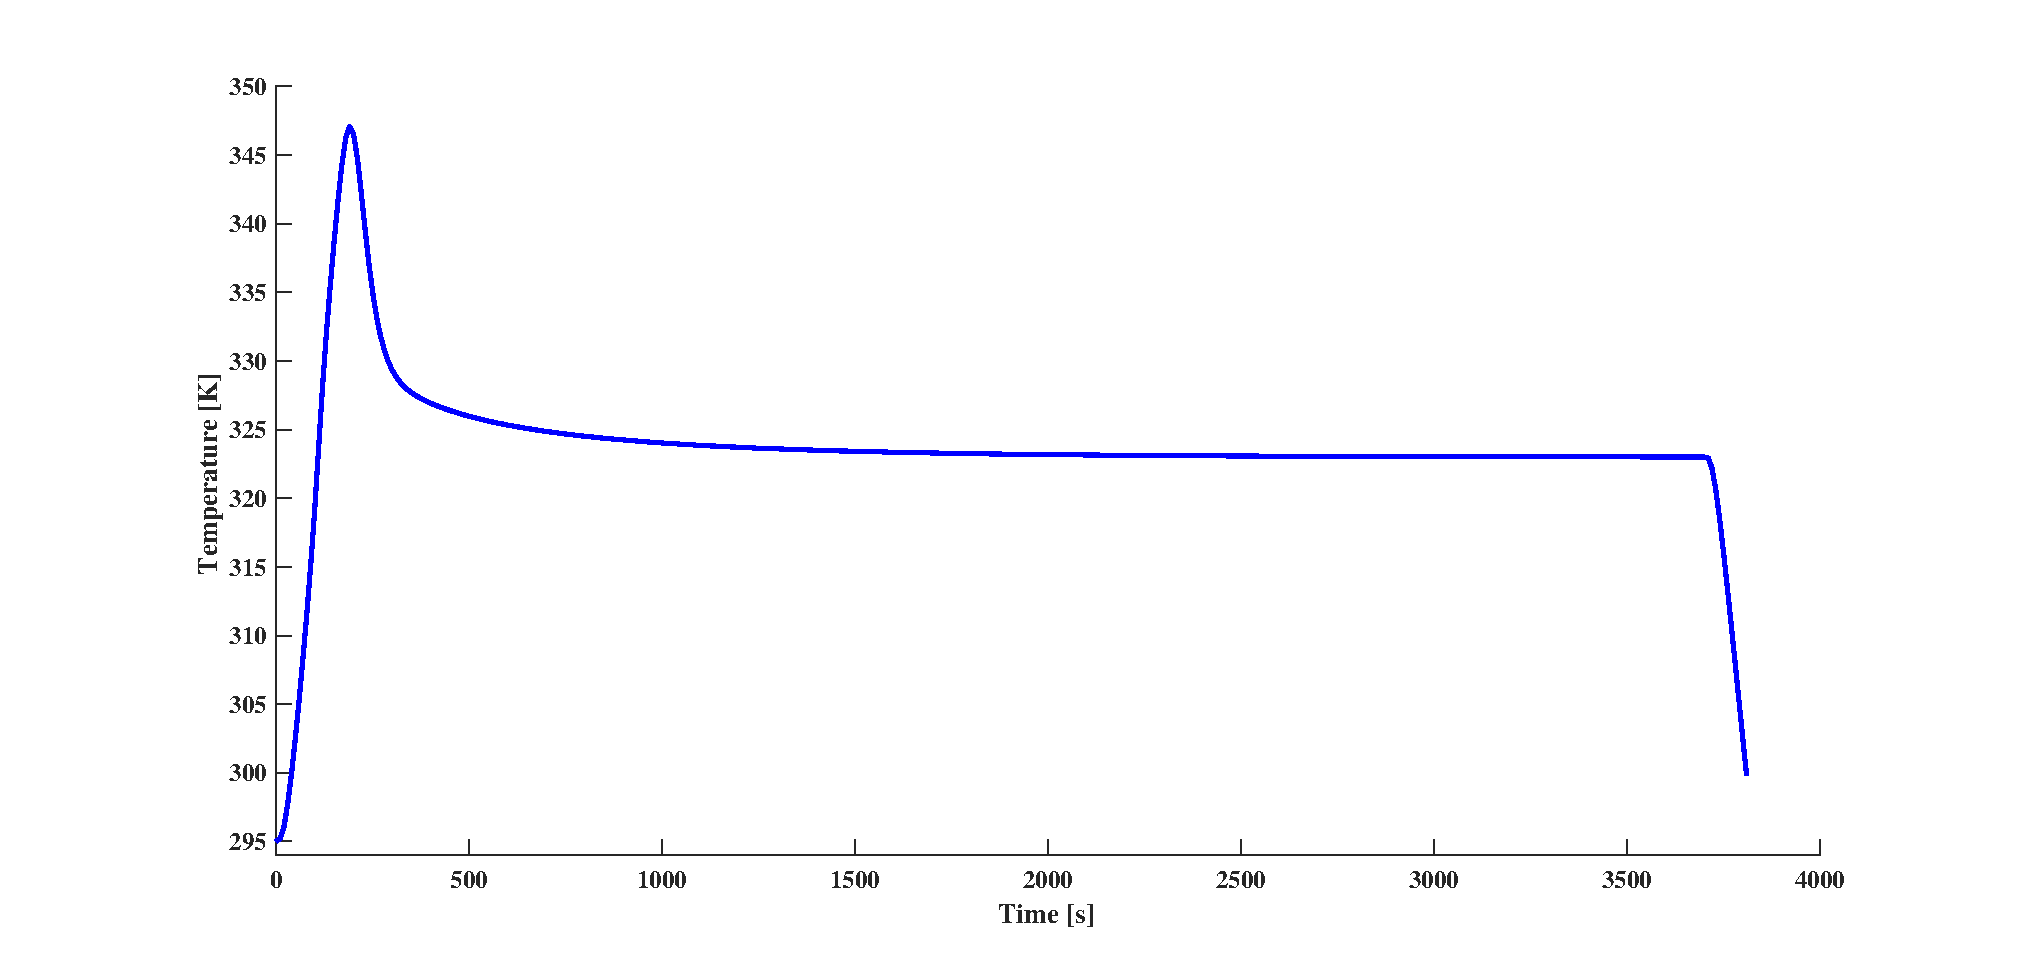
\includegraphics[width=0.9\textwidth]{obrazky/T-t.eps}
	\caption[Temperature evolution]{Temperature evolution in the cube center.}\label{obr:Curing_temperature}
\end{figure}

\begin{figure}[h!]
	\centering
	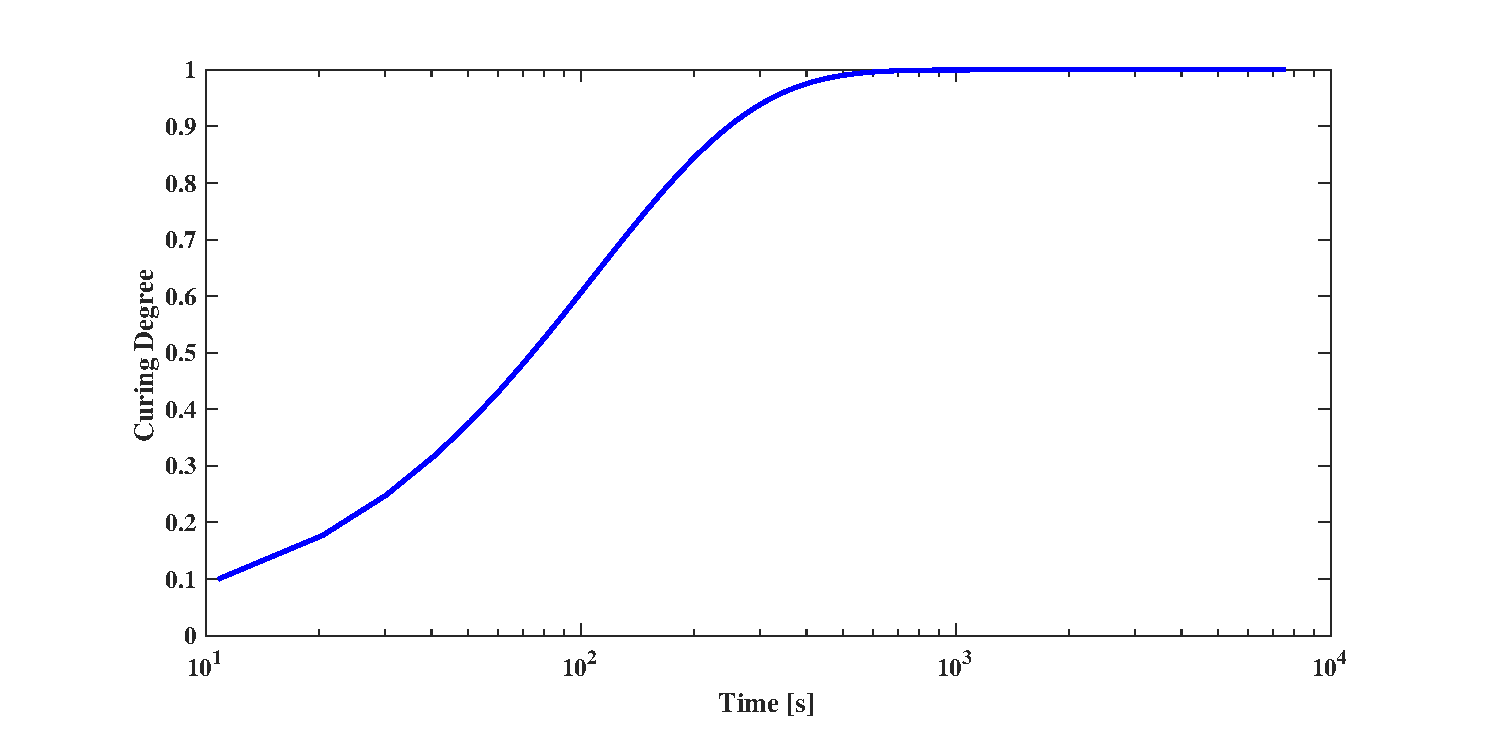
\includegraphics[width=0.9\textwidth]{obrazky/CD-t.eps}
	\caption[Degree of cure with respect to time]{Degree of cure with respect to logarithmic time.}\label{obr:Curing_curing}
\end{figure}

